\documentclass[a4paper,11pt]{report}
\usepackage[T1]{fontenc}
\usepackage{fourier}
\usepackage[utf8]{inputenc}
\usepackage[french]{babel}
\usepackage{hyperref}
\usepackage{biblatex}
\usepackage{xcolor}
\usepackage[scale=0.8]{geometry}
\usepackage{graphicx}

\usepackage{listings}
\lstset{basicstyle=\ttfamily,
  showstringspaces=false,
  basicstyle=\footnotesize\ttfamily,
  keywordstyle=\bfseries\color{green!40!black},
  commentstyle=\color{purple!40!black},
  identifierstyle=\color{blue},
  stringstyle=\color{red},
  breaklines=true,
  frame=l, % single, L, lines
  framerule=2pt
}

\colorlet{punct}{red!60!black}
\definecolor{background}{HTML}{FFFFFF}
\definecolor{delim}{RGB}{20,105,176}
\colorlet{numb}{magenta!60!black}
\lstdefinelanguage{json}{
    basicstyle=\normalfont\ttfamily,
    numbers=left,
    numberstyle=\scriptsize,
    stepnumber=1,
    numbersep=8pt,
    showstringspaces=false,
    breaklines=true,
    frame=lines,
    backgroundcolor=\color{background},
    literate=
     *{0}{{{\color{numb}0}}}{1}
      {1}{{{\color{numb}1}}}{1}
      {2}{{{\color{numb}2}}}{1}
      {3}{{{\color{numb}3}}}{1}
      {4}{{{\color{numb}4}}}{1}
      {5}{{{\color{numb}5}}}{1}
      {6}{{{\color{numb}6}}}{1}
      {7}{{{\color{numb}7}}}{1}
      {8}{{{\color{numb}8}}}{1}
      {9}{{{\color{numb}9}}}{1}
      {:}{{{\color{punct}{:}}}}{1}
      {,}{{{\color{punct}{,}}}}{1}
      {\{}{{{\color{delim}{\{}}}}{1}
      {\}}{{{\color{delim}{\}}}}}{1}
      {[}{{{\color{delim}{[}}}}{1}
      {]}{{{\color{delim}{]}}}}{1},
}
\lstdefinelanguage{javascript}{
  keywords={break, case, catch, continue, debugger, default, delete, do, else, finally, for, function, if, in, instanceof, new, return, switch, this, throw, try, typeof, var, void, while, with},
  morecomment=[l]{//},
  morecomment=[s]{/*}{*/},
  morestring=[b]',
  morestring=[b]",
  sensitive=true
}

\usepackage{lastpage}
\usepackage{fancyhdr}


\cfoot{\thepage\ of \pageref{LastPage}}

% \fancyhead{} % clear all header fields
% \fancyhead[C]{\scriptsize Notre beau titre}
% \fancyfoot{}
% \fancyfoot[C]{\thepage/\pageref{LastPage}} % clear all footer fields
% %\fancyfoot[LE,RO]{}
% %\fancyfoot[RE,LO]{\scriptsize Webs'INT - Télécom SudParis}
% \fancyfoot[CO,RE]{}
% %\renewcommand{\headrulewidth}{0pt}
% %\renewcommand{\footrulewidth}{0pt}



\title{Environnements de TP pour MOOC}
\author{François Monniot \& Alexis Mousset}

% PDF metadata
\hypersetup{pdfinfo={
  Author={François Monniot, Alexis Mousset},
  Title={Adding PDF metadata in LaTeX},
  Keywords={MOOC;Docker;TSP}
}}

\addbibresource{report.bib}


\begin{document}

\maketitle
\tableofcontents

\begin{abstract}

\end{abstract}
\pagestyle{fancy}
\chapter{Introduction}
\pagestyle{fancy}
\section{MOOC}

\subsection{Contexte des MOOC à TSP et en général}

\subsection{Contexte des besoins de TP}

\section{Docker}

\subsection{Expression précise du besoin}

Le besoin exprimé dans le cadre de notre projet de fin d'études est la gestion d'environnements de travaux pratiques pour des MOOC, notamment les MOOC mis en place à Télécom SudParis. Un environnement de TP est déjà en place pour le MOOC de bases de données, basé sur Vagrant.

Ces environnements doivent pourvoir êtres utilisés sur les postes des apprenants, et éventuellement aussi sur un serveur. Cela impose plusieurs contraintes :
\begin{itemize}
  \item Compatibilité logicielle : utilisable sur la grande majorité de systèmes d'exploitation, même dans des version anciennes
  \item Compatibilité matérielle : utilisable sur du matériel ancien et peu performant
\end{itemize}

Ces environnements doivent aussi être faciles à créer et ne nécessitent que peu de compétences
particulières.

\subsection{Qu'est-ce que Docker ?}

Docker\cite{website:whatis-docker} a été lancé en tant que projet open-source en mars 2013.
C'est un programme permettant de gérer le déploiement d'un type de virtualisation particulier : les conteneurs.
  
\subsection{Adéquation de la solution}

Utilisation de boot2docker, qui installe VirtualBox, MSYS-git

tiny core linux : 27MB de RAM dans  boot2docker

Par rapport à Vagrant :
\begin{itemize}
  \item Mêmes besoins matériels : support de la virtualisation, 2 Go de RAM pour un usage confortable.
  \item Le principal obstacle au niveau compatibilité est la nécessité d'un OS 64 bit.
  \item Au niveau professeur, utilisation de scripts pour la mise en place. Facilité de migration vers Docker.
  \item Au niveau apprenant, installation légèrement plus simple (boot2docker), et mise à jour facilitée en utilisant les mises à jour incrémentales des images docker.
  \item Plus orienté production si utilisation sur un serveur.
\end{itemize}

\subsubsection{Compatibilité logicielle}

Docker nécessite en général un noyau linux supérieur à 3.8 (sorti en février 2013) à cause d'un bug LXC\cite{website:bug-lxc} présent dans les versions antérieures, ainsi qu'un noyau 64 bit.

Distribution pleinement compatibles :
\begin{itemize}
  \item Ubuntu à partir de la 13.04, notamment Ubuntu 14.04 LTS.
  \item Debian à partir de la version 8
  \item RHEL/CentOS à partir de la version 7
  \item RHEL à partir de la version 6.5 avec un noyau supérieur à 2.6.32-431, qui contient le patch nécessaire à Docker. Docker doit être installé de puis les dépôts EPEL.
\end{itemize}

Distribution compatibles après adaptations :
\begin{itemize}
  \item Ubuntu 12.04 LTS (kernel backporté)
  \item Debian 7 (kernel backporté)
  \item RHEL 6 à partir de la version 6.5 avec un noyau supérieur à 2.6.32-431, qui contient le patch nécessaire à Docker (docker doit être installé de puis les dépôts EPEL)
\end{itemize}

Un résumé de la compatibilité est présenté dans le tableau \ref{tab-linux}.

\begin{figure}[h!]
\begin{center}
  \begin{tabular}{| c | c | c | }
     \hline
     Distribution & Support natif & Support après adaptation \\ \hline
     Debian & 8 (jessie) & 7 (wheezy) \\ \hline
     Ubuntu & 13.04, 13.10, 14.04 LTS, 14.10 & 12.04 LTS \\ \hline
     RHEL/CentOS & 7 & 6.5, 6.6 \\
     \hline
   \end{tabular}
      \end{center}
  \caption{Compatibilité logicielle de Docker sous Linux}
  \label{tab-linux}
\end{figure}

En cas de problème de version kernel, il est possible d'utiliser la même méthode que boot2docker et installer une VM utilisant un noyau récent (par exemple un CoreOS).

Sous Windows et MacOS, la compatibilité est celle de VirtualBox (à partir de Windows XP), avec la contrainte supplémentaire d'un OS 64 bit, ce qui en pratique ne retient que les systèmes postérieurs à Windows Vista (surtout à partir de Windows 7) et Mac OS X 10.5. 

\subsubsection{Compatibilité matérielle}

Comme toute solution basée sur la virtualisation, l'utilisation nécessite un processeur avec support de la virtualisation matérielle. Boot2docker demande aussi un minimum de 2Go de RAM.

Docker nécessitant un hôte 64bit, l'hôte de boot2docker doit aussi être en 64bit. En général la limitation est logicielle, les processeurs supportant la virtualisation étant en général en 64bit. Les processeurs 64bit recouvrent les processeurs :

\begin{itemize}
  \item AMD à partir de 2003 avec les Opteron et Athlon 64
  \item Intel à partir de 2004 avec certains Pentium 4 et Xeon, sauf Atom et Celeron jusqu'à 2008.
\end{itemize}

Le tableau \ref{compat} résume la compatibilité des environnements basés sur docker.

   \begin{figure}[h!]
\begin{center}
   \begin{tabular}{| c | c |}
     \hline
     Caractéristique & Minimum \\ \hline
     RAM & 2Go \\ \hline
     Disque & 1Go disponible \\ \hline
     Mac OS X & 10.5 en \textbf{64 bit} \\ \hline
     Linux & 3.8 et 2.6.32-431 RHEL en \textbf{64 bit} \\ \hline
     Windows & (Vista), 7, 8, 8.1 en \textbf{64 bit} \\
     \hline
   \end{tabular}
   \end{center}
   \caption{Compatibilité matérielle et logicielle}
   \label{compat}
  
\end{figure}

\chapter{Implémentation}

Le projet est open source et a été développé publiquement. Ainsi tout les codes sources sont disponible sur GitHub et sont regroupé dans l'organisation «pfe-asr-2014». On peut y retrouver les codes sources bien entendue, mais également documentation et tests. Enfin le projet dispose de son propre site web à l'adresse pfe-asr-2014.github.io.

\section{Architecture}

La platforme que nous proposons est basé sur des conteneurs Docker. Ainsi chaque composant peut, dans l'absolu, être utilisé de manière
completement indépendante les uns des autres. La figure~\ref{architecture} représente l'architecture telle qu'envisagée lors de ce projet.

\begin{figure}[h]
   \caption{\label{architecture} Architecture de la plateforme}
   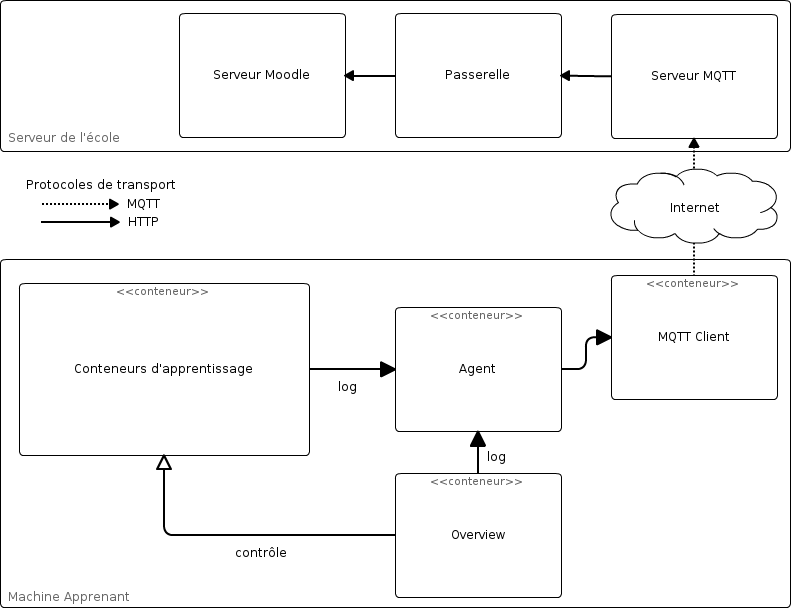
\includegraphics[width=\textwidth, keepaspectratio=true]{architecture.png}
\end{figure}

Cette architecture se décompose en deux parties principales: la première est gérer par l'école et peut se déployer sur des serveurs dédiés ou sur un cloud; la deuxième partie est basé sur docker et peut donc être déployé dans n'importe quel environnement docker (c'est d'ailleurs une des grandes force de docker), dans notre cas il s'agit couramment de l'ordinateur de l'apprenant mais on peut envisager la possibilité d'héberger ces conteneurs sur un cloud gérer par l'école et directement proposer les accés aux apprenants.

La communication entre les groupes est assuré via l'utilisation du protocole MQ Telemetry Transport (MQTT). Il s'agit d'un protocole de communication prévu pour ne pas consommer beaucoup de ressources (il est par exemple utilisé dans l'embarqué, l'internet des objets mais aussi la communication avec des satellites) et qui est résilient. Il offre un minimum de fonctionnalité (publish/subscribe) ce qui nous suffit, nous l'avons choisi car il permet d'avoir une faible emprunte sur des machines de faible puissance que certains des apprenants peuvent utiliser.

\subsection{Serveur}

Le serveur fonctionne avec trois briques logiciels différents:

\begin{itemize}
  \item Un plugin moodle qui permet l'enregistrement des traces des apprenants dans le système moodle afin de permettre aux professeurs de créer des rapports.
  \item Une passerelle entre le serveur MQTT et moodle qui transforme les données obtenu via MQTT dans un format reconnu par moodle.
  \item Un serveur (broker) MQTT sur lequel les brokers distant vont se connecter pour transmettre les traces qu'ils auront genérer.
\end{itemize}

Ces trois briques logiciels peuvent être déployer sur différents serveurs si l'on a besoin de répartir la charge. Nous recommandons dans ce cas de grouper la passerelle et le broker MQTT sur une même machine qu'il suffit de multiplier pour passer à l'échelle.

\subsection{Apprenant}

Le coté apprenant est composé de deux conteneurs essentiels si déployer sur un cloud:

\begin{itemize}
  \item Le broker MQTT qui permet de transmettre les traces des apprenants au serveur distant.
  \item Et l'agent qui collecte les traces des apprenants émis par les conteneurs de cours, les mets en forme et les retransmets au broker MQTT.
\end{itemize}

Si l'environnement est disponible sur la machine de l'apprenant alors le conteneur Overview permet de fournir une interface graphique qui permet gérer les conteneurs d'apprentissages de manières extremement simple.

Enfin des conteneurs d'apprentissages composent les environnement des travaux pratiques des apprenants, ils fournissent les éléments essentiels à la réalisation des travaux pratiques et permettent de remonter, de façon anonyme ou non, des informations sur leurs utilisation, l'avancement de l'apprenant voir des résultats d'examen.

\section{Agent}

\section{Moodle}

Afin de pouvoir insérer les informations relatives aux travaux pratiques dans le système moodle il nous faut une porte d'entrée dans le-dit système. Il n'existe malheureusement pas de façon simple de fournir ces informations à moodle (c'est-à-dire sans développer un plugin spécifique).
C'est donc ce que nous avons fait. Le plugin développer est très simple dans son utilisation: après installation du plugin et identification de l'utilisateur, il est possible via une simple requête HTTP de fournir à moodle un «évènement». La figure~\ref{seq-submit-event} ci-après représente la manière de soumettre un évènement.

\begin{figure}[h]
   \caption{\label{seq-submit-event} Diagramme de séquence de la soumission d'un évènement}
   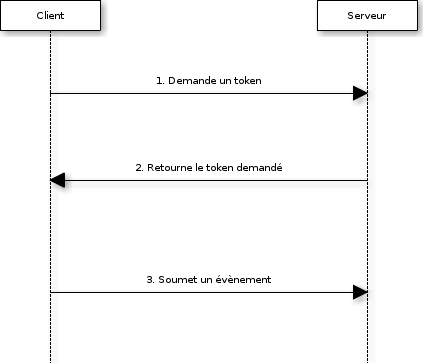
\includegraphics[width=8cm, keepaspectratio=true]{mem-seq-submit-event.png}
\end{figure}

Comme visible dans la figure~\ref{seq-submit-event}, le procédé se fait en deux requêtes HTTP. La première est faite de la manière suivante:

\begin{lstlisting}[caption={Requête d'un token}]
GET http://localhost:8080/login/token.php?
  service=mem&
  username=&
  password=
\end{lstlisting}

Il faut que les champs «username» et «password» soit complété avec le nom d'utilisateur et le mot de passe du compte moodle de l'apprenant.
Moodle renvoie alors le token avec la réponse au format json suivante:

\begin{lstlisting}[language=json, caption={Retourne le token}]
{"token":"le token de l'utilisateur"}
\end{lstlisting}

Maintenant que nous avons la possibilité de prouver que nous sommes bien un utilisateur nous pouvons envoyer un évènement à moodle via la requête HTTP suivante:

\begin{lstlisting}[caption={Soumet un évènement}]
POST http://localhost:8080/webservice/rest/server.php?
    wsfunction=local_mem_post_event&
    wstoken=<token de l'utilisateur>&
    moodlewsrestformat=json&
    category="mooc"&
    action="begin"&
    label="Relational Database"&
    datetime="2014-12-11T16:31:12.436+01:00"
\end{lstlisting}

Les quatres dernier champs sont les plus importants: la catégorie, l'action, le label et le temps permettent de spécifier un évènement. Avec une combinaison de ces quatres valeurs, on peut décrire tous les évènements produits par les apprenants. Par exemple dans la requête précédente nous avons soumis un évènement concernant le début du cours concernant les bases de données relationnels, de plus l'apprenant à commencer ce cours le 11 décembre en fin d'après-midi (16h30).
Le format de description est suffisament générique pour qu'il puisse décrire un évènement métier (début d'un cours) ou un évènement technique (soumission d'une requête SQL) tout en gardant un format unique dans les différents cas. Si le format d'évènement choisi avait été moins générique, il aurait falu en maintenir plusieurs suivant le type d'information à transmettre ce qui aurait augmenter la complexité du système sans gain significatif.

\section{tracker.js}

L'interet de la nouvelle plateforme de MOOC c'est d'etre capable de fournir aux enseignants des retours sur ce qu'on fait les apprenants. Ainsi des questions comme «Est-ce que le TP a la bonne difficulté ?» ou «Pourquoi est-ce que la majorité des apprenants se trompent à la question 5?» peuvent trouver une réponse dans le comportement des apprenants (par exemple, la majorité des réponses sont les mêmes, la question posée est-peut être mal formulé). Aussi faut-il connaitre les actions des apprenants lorqu'ils réalisent le TP.
C'est pour répondre à cette problèmatique qu'est née tracker.js.

Tracker.js est une simple bibliothèque javascript à intégré dans une page web et qui permet de déclarer un certain nombre d'évènement à surveiller.
De maniere pratique cela permet d'enregistrer les cliques de souris, les frappes clavier ou un évènement personalisé et d'envoyer les informations à l'agent pour qu'il relais les informations à moodle.

Le tracker à été écrit de manière à promouvoir une API simple et concise, ainsi on obtient une déclaration simple et trés lisible des évènements:

\begin{lstlisting}[language=javascript, caption={Exemple d'utilisation de tracker.js}]
// Instanciation du tracker
var tracker = new Tracker({distant: 'url'});

// On ecoute les evenements "onclick" sur les elements de classe "my-element"
tracker.on('.my-element').track('click');
\end{lstlisting}


\section{Overview}

Overview est un site web fournissant à l'apprenant une interface graphique pour gérer les conteneurs d'apprentissage sur son ordinateur personelle.
En effet, certain cours comme les bases de données relationnel n'ont pas de réel lien avec la ligne de commande UNIX. Dès lors, le pré-requis de savoir utiliser la ligne de commande pour pouvoir effectuer le TP de base de donnée est un frein pour un certain nombre d'apprenant. Overview permet de se passer de cette difficulté.

Overview est composé de deux composants relativement indépendant: un serveur backend écrit en Python avec le framework flask et une interface frontend qui effectue des requêtes REST au serveur.

\subsection{Frontend}

D'un point de vue utilisateur il s'agit d'un simple site web qui propose, pour chaque cours disponible, quatres actions: installer, désinstaller, démarrer et arrêter. Ces actions sont conditionnelles: lorsqu'un conteneur est démarré on ne propose pas les actions «installer» et «démarrer» qui n'aurait pas de réel sens dans le contexte.

Le code javascript à été écrit pour être facilement testable et modulable. Il se décompose en plusieurs module (ou fichier):

\begin{itemize}
  \item \textbf{log.js} Bibliothèque développé par Adam Schwartz est qui fourni plusieurs amélioration pour journaliser des informations (notament l'utilisation du markdown ou l'affichage de code).
  \item \textbf{api.js} Un objet permettant d'abstraire les appels au serveur via une interface implémentant la «Désignation chainée». Ainsi une requête PATCH à notre serveur avec un objet quelconque s'effectue avec le code suivant:
    \begin{lstlisting}[language=javascript,caption={Requête PATCH à l'api}]
    var api = new Api('http://mon-serveur.com/api/v1/');
    api.patch('services/'+serviceId).with(quelconque).now(function(status, data){});
    \end{lstlisting}
    L'objet «quelconque» ici passé en paramètre sera transformé en JSON et passé dans le corps de la requête. La fonction passé à «now» sera executé lors de la reception de la réponse du serveur avec le statut HTTP et les données de la réponse. Il est a noté qu'il n'a pas été jugé utile de retourner les en-têtes HTTP dans la fonction de rappel. La connexion avec le serveur est réalisé avec l'objet XMLHttpRequest qui fait partie des spécifications javascript et est disponible sur tous les navigateurs «modernes».
  \item \textbf{router.js} Cet objet permet d'écouter les changements d'adresse du navigateur et de réagir en consèquence. Plus précisemment, le frontend utilise les «hash» de l'URL afin de savoir les actions qu'il faut exécuter. Les hash sont les caractères situé après le dièse de l'URL, par exemple dans l'URL http://monsite.com/\#pub, «pub» est le hash.
  Le routeur permet d'enregistrer des actions à réaliser lorsque le hash correspond à un schéma prédéfinni. Ce schéma est composé d'une action (une chaine de caractère choisi par le développeur qui ne peut comporter le signe «:» (utilisé comme délimiteur) et qui respecte les standards définissant une URI; la deuxième partie du schéma sera l'identifiant du cours (appelé «service» dans le code et la documentation).
  Un exemple étant plus parlant, voici le code qui permet d'afficher l'identifiant d'un cours lorsque le hash est «show:my-cours-id»:
    \begin{lstlisting}[language=javascript,caption={Affichage identifiant avec le routeur}]
    var router = new Router();
    router.register('show', function(serviceId){
      alert(serviceId);
    });
    \end{lstlisting}
  \item \textbf{drawer.js} qui permet d'ouvrir et de fermer le menu gauche pour gagner de la place et \textbf{table.js} qui re-organise le tableau sur mobile afin de garder la lisibilité.
  \item \textbf{main.js} Ce fichier n'est pas un module en soit mais déclare la logique du site web. C'est la glue qui relie tout les composants vue précédemment. On y déclare les états possible, les opérations à faire (routing) ainsi que certaines amélioration lié au design (barre de progression, action disponible et affiché à l'apprenant).
\end{itemize}

De plus, les modules \textbf{Router} et \textbf{Api} dispose de tests unitaire réalisé avec le framework \textbf{Jasmine.js}.

\subsection{Backend}

Le backend est développé en Python avec le framework Flask. Il se compose de quatres modules complèmentaires (représentation UML figure~\ref{uml-overview-module}):

\begin{itemize}
  \item \textbf{services} est une classe regroupant la gestion des services (les cours sont des services apparant à l'apprenant)
  \item \textbf{api} contient toutes les déclarations de route concernant l'api du serveur. C'est une passerelle entre l'utilisateur et la classe Services.
  \item \textbf{frontend} est le pendant de api pour servir les pages web. Il permet de servir la page web de Overview.
  \item \textbf{helpers} Contient des fonctions utilisées dans les templates web pour simplifier le code.
  \item \textbf{overview} Il s'agit du module python qui compose et crée l'application flask.
\end{itemize}

\begin{figure}[h]
   \caption{\label{uml-overview-module} Représentation UML du serveur Overview}
   \centering
   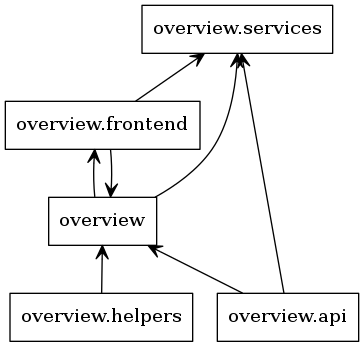
\includegraphics[scale=0.8, keepaspectratio=true]{packages_overview.png}
\end{figure}

Les liens bidirectionnel sont expliqué par le fait que le module overview importe frontend et api après avoir créé l'application flask et que ces deux modules utilise cette application flask pour la configurer. Cette organisation à été choisi pour séparer les roles de chacun (separation of concerns) et faciliter les tests. L'application est d'ailleurs entièrement couvert par des tests unitaires réalisé avec la bibliothèque standard de python et du collecteur noses.

L'API d'overview est sous la forme d'une API REST. Elle propose trois \textit{endpoint}:
\begin{itemize}
  \item \textbf{GET /api/v1/docker} permet d'obtenir l'état des conteneurs docker liés aux moocs TSP (on ne peut connaitre l'état des conteneurs n'ayant pas de rapport avec les moocs tsp).
  \item \textbf{GET /api/v1/services} permet d'obtenir l'état des services (nom, identifiant, état).
  \item \textbf{PATCH /api/v1/services/<service\_id>} permet de changer l'état d'un service.
\end{itemize}

Overview est basé sur des services. Un service c'est un ensemble de conteneur associé à une certaine configuration. Par exemple le cours de base de donnée est représenté par la configuration suivante:
\begin{lstlisting}[caption={Configuration du service mooc-db}]
- id: tsp-mooc-db
  completeName: Relational Database
  port: 8080
  stack:
    - containerName: tsp-moocdb-postgres
      image: fmonniot/tsp-moocdb-postgres:latest
    - containerName: tsp-moocdb-web
      image: fmonniot/tsp-moocdb-web:latest
      ports:
        - "8080:80"
      links:
        - tsp-moocdb-postgres
\end{lstlisting}

Cette configuration spécifie un identifiant (id), un nom lisible pour l'apprenant (completeName) ainsi qu'un port à exposer pour l'interface web. On remarque ensuite une section «stack»: il s'agit de la configuration des conteneurs docker. Chaque entrée correspond à un conteneur. Dans notre exemple nous avons un premier conteneur contenant la base de donnée postgreSQL et un second contenant l'interface graphique, lié à la base de donnée via un lien docker et exposant le port 8080 à l'utilisateur.

Afin de pouvoir gérer ces services, on introduit la notion d'état desdits services: ils peuvent être dans six états différents comme décrit par la figure~\ref{overview-states}. Les états «NOT\_INSTALLED», «STOPPED» et «RUNNING» ne change pas sans actions de l'utilisateur. Au contraire les états «INSTALLING», «STOPPING» et «UNINSTALLING» sont temporaires et changeront dès que leur action sera terminée.


\begin{figure}[h]
   \caption{\label{overview-states} Cycle de vie d'un service}
   \centering
   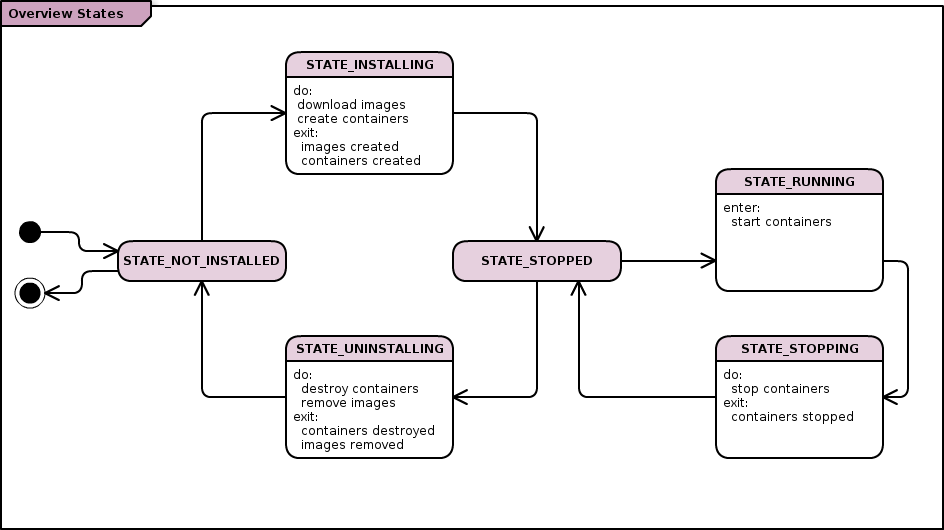
\includegraphics[width=\textwidth, keepaspectratio=true]{overview-states.png}
\end{figure}

\pagestyle{fancy}

\chapter{Utilisation}

\pagestyle{fancy}

\section{Cas d'utilisation : Le MOOC bases de données}

\subsection{Côté professeur}

L'objectif côté professeur est de faciliter la mise en place d'environnements de TP par des non spécialistes de docker (éventuellement assistés en cas de problèmes).
La configuration des machines de TP s'effectue sur un dépôt git contenant les scripts de création des environnements, ainsi que les contenus qui y seront ajoutés. Les images sont ensuite générées et déposées.
Le format de configuration est le Dockerfile, qui est constitué d'une suite de commandes lancées et de copies de fichiers. Il est très simple, si on sait configurer un système, de le consigner dans un Dockerfile.

La mise en place des TP de ce MOOC nécessite deux conteneurs : un pour la base de données et un pour le serveur et les applications web, ainsi que du conteneur permettant le suivi.

\begin{lstlisting}[language=Bash,caption={Dockerfile de base}]
RUN apt-get update && apt-get install my_software
COPY configuration_file /etc/my_software/
EXPOSE 80
# The command that should be executed
CMD ["/usr/bin/my_software"]
\end{lstlisting}

Le conteneur de base de données est basé sur l'image postgreSQL officielle (elle même basée
sur Debian). La configuration et le peuplement des bases de données sont effectuées à partir d'un script shell appelé lors de la création du conteneur. Ce script appelle les scripts de peuplement sql, et permet de créer les utilisateurs nécessaires.

L'image web est basée sur debian, sur laquelle est installée apache et phppgadmin. De plus des fichiers suppmémentaire sont ajoutés dans un autre virtualhost, qui contient donc les fichiers applicatifs liés au TP.

Une fois le container lancé, l'insterface web est accessible en local sur la machine.

\subsection{Côté apprenant}

L'apprenant doit d'abord installer boot2docker, qui se charge d'installer git et virtualbox s'ils ne sont pas présents. Le téléchargement est de 122 Mo. L'installeur ajoute un raccourci dans les menus permettant d'accéder à un shell sur le VM boot2docker, sans avoir à passer par virtualbox. Ensuite l'apprenant doit exécuter des commandes permettant de récupérer les images correspondant à son TP, puis à les lancer. Il peut ensuite accéder à sont environnement de TP.

% todo : doc apprenant

overview ?


\printbibliography

\end{document}
